%**********************************************************
\subsection{Task Overview}
One can define and describe briefly how the gateway is implemented, making use of threads and processes.

\begin{itemize}
	\item \textbf{tLoraRecv:}
	\item \textbf{tLoraSend:}
	\item \textbf{tTCPSend:} sends a message to the remote server, via TCP/IP communication protocol;
	\item \textbf{tTCPRecv:} receives a message from the remote server, via TCP/IP communication protocol.
\end{itemize}

%**********************************************************
\subsection{Task Priority}

%**********************************************************
\subsection{Task Synchronization}

\myparagraph{Condition Variables}
The condition variables used in this system are listed below.

\begin{itemize}
	\item \textbf{condLoraSend:}
	
	\item \textbf{condTCPSend:} used to notify \textit{tTCPSend} that a new message is ready to be sent;
		
\end{itemize}

\myparagraph{Mutexes}
The mutexes used in this system are listed bellow.

\begin{itemize}
	\item \textbf{mutLoraComm:}
	\item \textbf{mutLoraSend:}	
	
	\item \textbf{mutTCPComm:} mutex used to protect the TCP/IP communications (send and receive);
	\item \textbf{mutTCPSend:} mutex associated with the condition variable \textit{condTCPSend} to send a message via TCP/IP protocol communication;
\end{itemize}

%\myparagraph{Semaphores}

%\subsection{Task Communication}
%\myparagraph{Message Queues}
%\myparagraph{Signals}

%**********************************************************
\subsection{Flowcharts}
\myparagraph{tLoraRecv}
This task, presented in figure \ref{fig:gwtLoraRecv}, is responsible for receiving all the packets sent by the local systems, through LoRa communication. This task makes use of a mutex \textit{mutLoraComm}, to protect LoRa send and receive functions, which must not occur at the same time.

When a message is received it is pushed into a vector of messages, to be sent to the remote system, named \textit{msgs\_to\_rs}. This way, we can receive continually messages from local systems, while there is another task sending this messages.

\begin{figure}[H]
	\centering
%	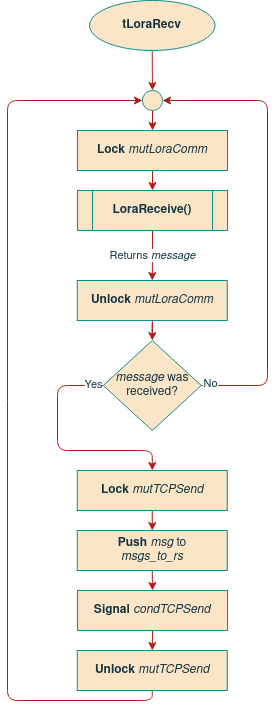
\includegraphics[width=.65\textwidth]{09sw_specification/gwtLoraRecv}
	\caption{Flowchart: Gateway tLoraRecv.}
	\label{fig:gwtLoraRecv}
\end{figure}

\myparagraph{tLoraSend}
This task, presented in figure \ref{fig:gwtLoraSend}, is responsible for sending all the packets sent by the remote system to the local systems. In addiction to the mutex \textit{mutLoraComm}, this task makes use of another mutex \textit{mutLoraSend}, which comes along with the condition variable \textit{condLoraSend}, in order to protect the insertion and removal of messages from the vector \textit{msgs\_to\_ls}.

When there are no messages to send to the local systems, i.e, the messages vector \textit{msgs\_to\_ls} is empty, then the task enters a sleep state, waiting for \textit{condLoraSend} to be notified. When this happens, the mutex that protects LoRa communication is locked and a message is popped from the queue of messages to being sent to the local systems. If the vector \textit{msgs\_to\_ls} is not empty after sending a message, this task continues to do so until there are no more to send, before entering into sleep state again.

\begin{figure}[H]
	\centering
	%	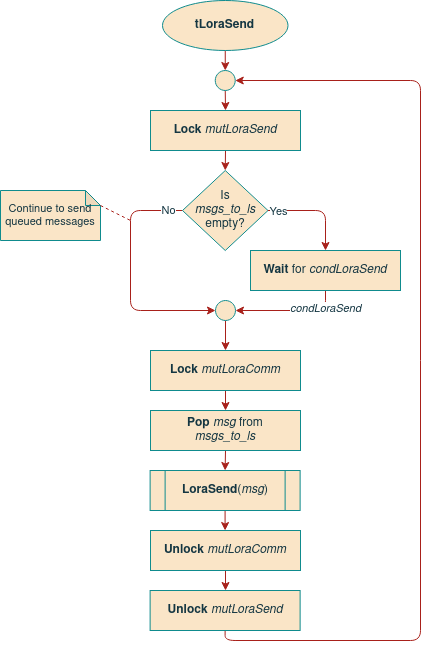
\includegraphics[width=.65\textwidth]{09sw_specification/gwtLoraSend}
	\caption{Flowchart: Gateway tLoraSend.}
	\label{fig:gwtLoraSend}
\end{figure}

\myparagraph{tTCPSend}
This task, presented in figure \ref{fig:gwtTCPSend}, is responsible for sending all the messages sent by the local systems to the remote system, being received by in the task \textit{tLoraRecv}. It uses two mutexes: \textit{mutTCPSend} associated with the condition variable \textit{condTCPSend}, that synchronizes the insertion and removal of the messages from the vector \textit{msgs\_to\_rs}; and \textit{mutTCPComm}, to protect the communications send and receive.

When there are no messages to send to the remote system, i.e, the messages vector \textit{msgs\_to\_rs} is empty, the task enters a sleep state, waiting for \textit{condTCPSend} to be notified by the task receiving messages from the local systems. When messages are received, the vector \textit{msgs\_to\_rs} is not empty, and one can lock the mutex \textit{mutTCPSend} in order to pop a message from the vector. After that, one can send the message via TCP/IP communication protocol, protecting the communication with the mutex \textit{mutTCPComm}.

\begin{figure}[H]
	\centering
	%	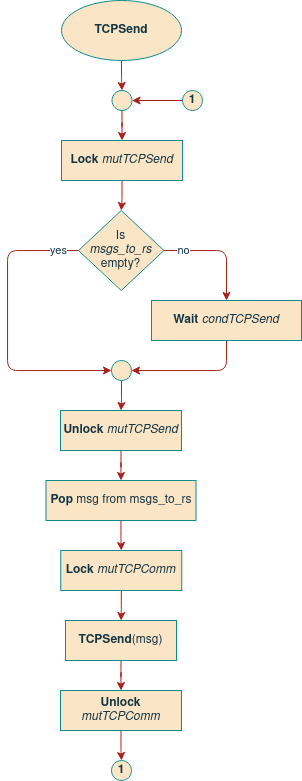
\includegraphics[width=.65\textwidth]{09sw_specification/gwtTCPSend}
	\caption{Flowchart: Gateway tTCPSend.}
	\label{fig:gwtTCPSend}
\end{figure}

\myparagraph{tTCPRecv}
This task, presented in figure \ref{fig:gwtTCPRecv}, is responsible for receiving the messages sent by the remote system to the local systems. Unlike the send tasks, this thread never enters the sleep state because we can receive a message at any moment, so first, one have to lock the mutex \textit{mutTCPComm} and try to receive a message. If it was received a message, i.e, the \textit{msg} variable is not empty, then one can push the message to the messages vector \textit{msgs\_to\_ls} and notify the condition variable \textit{condLoraSend}, after locking its mutex \textit{mutLoraSend}, to inform that a new message has been received.

\begin{figure}[H]
	\centering
	%	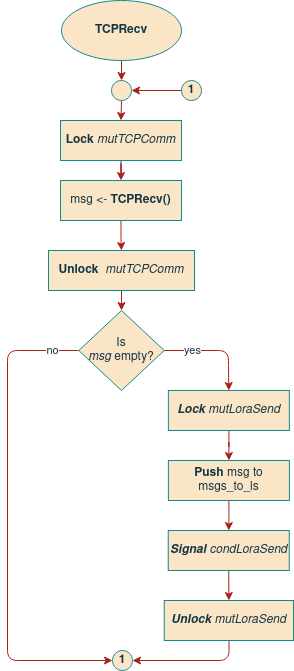
\includegraphics[width=.65\textwidth]{09sw_specification/gwtTCPRecv}
	\caption{Flowchart: Gateway tTCPRecv.}
	\label{fig:gwtTCPRecv}
\end{figure}

%**********************************************************
\subsection{Start-up Process}

%**********************************************************
\subsection{Shutdown Process}
